\documentclass[a4paper,10pt]{article}
\usepackage[utf8x]{inputenc}

\usepackage{graphics}
\usepackage{amsmath}    % need for subequations
\usepackage{graphicx}   % need for figures
\usepackage{verbatim}   % useful for program listings
\usepackage{color}      % use if color is used in text
\usepackage{subfigure}  % use for side-by-side figures
\usepackage{hyperref}   % use for hypertext links, including those to external


%% Encabezado y Pie de Pagina %%

\makeindex

%opening
\title{Computaci\'on Gr\'afica \\Texturas Procedurales \\Grupo 2}
\author{Guillermo Campelo\\Juan Ignacio Go\~ni\\Juan Tenaillon\\Santiago
V\'azquez}

\begin{document}

\maketitle

\begin{abstract}
Se agregó al motor de Ray Tracing, la posibilidad de utilizar texturas
procedurales.  Para lograr esto, se implementó Perlin Noise, y se implementaron
texturas que se asemejan al fuego, agua, granito, madera, mármol y material de
tipo orgánico para triángulos y esferas.
\end{abstract}

\section{Introducción}

A lo largo de este informe, detallaremos el diseño y desarrollo de la extensión
al motor de ray tracing.  Esta extensión consistió en agregar texturas
procedurales al motor, mediante la implementación de Perlin Noise.

Para realizar la extensión, partimos desde la base de la entrega anterior,
donde lo único que tuvimos que hacer fue implementar los nuevos
\textit{shaders}.

Para obtener los mismos resultados que obtiene Ken Perlin con su algoritmo de
texturas procedurales, realizarmos una investigación sobre los distintos típos
de ruidos que él utilizó, así como también con distintas fórmulas para aplicar
a ese ruido y obtener así las distintas texturas.

En la sección \ref{ruido} entraremos en más detalle con respecto a los posibles
ruidos, en la sección \ref{texturas} comenzaremos a explicar cada textura en
particular, mostrando cómo fue lograda y mostrando ejemplos de la misma.  En la
sección \ref{representacion} mostraremos cómo decidimos representar los
distintos shaders, y daremos valores recomendados para su uso. Por último,
comentaremos los resultados obtenidos así como nuestras conclusiones en la
sección \ref{conclusiones}.

\section{Ruido}
\label{ruido}
Como todos sabemos, la idea general de Perlin Noise es la de realizar sumas
sucesivas de ruidos a distintas amplitudes, para luego aplicarle a esa
sumatoria una función que nos determinará el color en el punto.

Entonces, es necesario definir primero el ruido para despues poder realizar las
sumas correspondientes.  Dentro de las posibilidades con las que nos
encontramos, resaltaban dos: Ruido Aleatorio y Ruido Mejorado.

\subsection{Ruido Aleatorio}

La idea de ruido aleatorio es básicamente esa.  Generamos una matriz de cierto
tamaño con número aleatorios entre 0 y 255.  De esta forma, se van a ir
realizando las sucesivas sumas y su resultado será nuevamente un número
aleatorio.

Esta fue la primera implementación de Ken Perlin, que luego fue suplantada por
el Ruido Mejorado que comentamos a continuación en la sección \ref{improved}.

\subsection{Ruido Mejorado}
\label{improved}

El ruido mejorado parte de la base del ruido aleatorio, originandose con un
vector de 256 valores aleatorios entre 0 y 255 inclusive.  Luego se crea otro
vector de permutación, que es luego utilizado para realizar las sumas de los
ruidos.

La ventaja que presenta este tipo de ruido con respecto al aleatorio, es que
este es más eficiente para los cálculos que realiza, obteniendo así una mejora
en el desempeño del algoritmo para generar las texturas.

Es debido a estas mejoras, presentadas por Ken Perlin en su paper ``Improving
Noise'', es que decidimos realizar la segunda implementación de ruido para
generar nuestras texturas.


\section{Texturas}
\label{texturas}

Las texturas que implementamos son las siguientes: fuego, agua, material
orgánico, piedra tipo granito, madera y marmol.  A continuación, mostraremos
para cada una de las texturas, la formula utilizada y el resultado obtenido.

\subsection{Fuego y Agua}

Para realizar la textura que simule al fuego y al agua, utilizamos la mísma
fórmula pero variando los colores aplicados.

La fórmula utilizada fue:

\begin{equation}
 sum (\frac{1}{f} * |Noise|) = |Fnoise(p)| + \frac{1}{2}|Fnoise(2p)| +
\frac{1}{4}|Fnoise(4p)| + ...
\end{equation}

Donde, $FNoise$ es la función que dado un punto $p$ me devuelve el ruido en ese
punto y donde $f$ es la frecuencia.  La idea sería realizar sumas sobre los
puntos, donde a medida que se hace más $profunda$ la suma van perdiendo fuerza
los términos y siempre tomando el valor absoluto.

En las figuras \ref{fig:figure1} y \ref{fig:figure2} se observa la textura
obtenida para simular fuego así como la textura obtenida para simular agua.

\begin{figure}[ht]
\begin{minipage}[b]{0.5\linewidth}
\centering
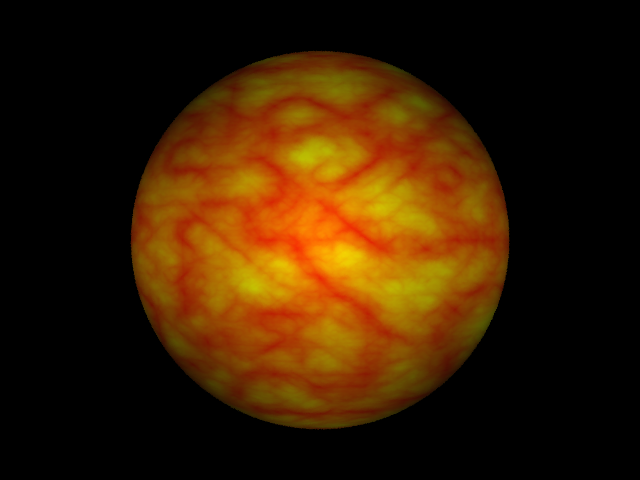
\includegraphics[scale=0.28]{proceduralFire.png}
\caption{Fuego Procedural}
\label{fig:figure1}
\end{minipage}
\hspace{0.5cm}
\begin{minipage}[b]{0.5\linewidth}
\centering
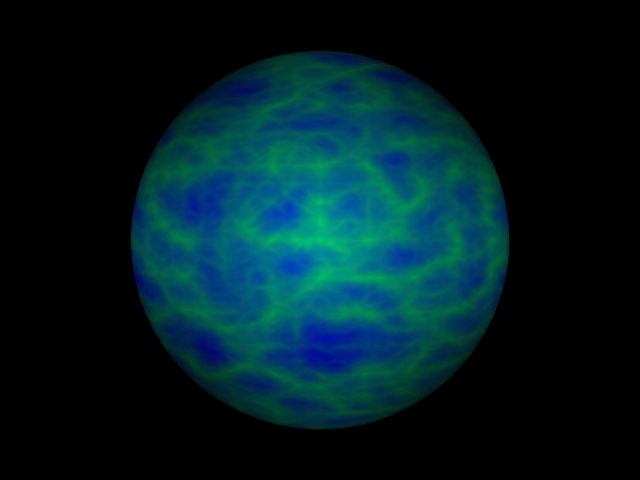
\includegraphics[scale=0.28]{proceduralWater.png}
\caption{Agua Procedural}
\label{fig:figure2}
\end{minipage}
\end{figure}

\subsection{Material Orgánico}

Para realizar una textura que simule a un material orgánico, tuvimos que
determinar primero que era un material orgánico y luego realizar
experimentaciones para obtener algo que lo simule.  Luego de realizar distintas
pruebas, y fallar en el intento, nos inclinamos por utilizar solamente la
función de ruido de perlin.

\begin{equation}
 Noise = Fnoise(p) + \frac{1}{2} Fnoise(2p) + ...
\end{equation}

De esta forma, lo que simulamos es una superficie con moho, un tipo de
hongos.  En la figura \ref{fig:figure3} se puede observar el resultado obtenido.

\begin{figure}[h!]
 \centering
 
\includegraphics[scale=0.5]{./proceduralOrganic.png}
 % proceduralOrganic.png: 640x480 pixel, 72dpi, 22.58x16.93 cm, bb=0 0 640 480
 \caption{Material Orgánico Procedural}
 \label{fig:figure3}
\end{figure}

\subsection{Piedra tipo Granito}

Esta textura fue otra de las que nos trajo aparejados cierto problemas.  Al
investigar la textura del granito, no lograbamos encontrar la fórmula que nos
permita simularlo.

Luego de intentar mediante prueba y error, advertimos que utilizando solamente
la función de ruido, pero escalandolo a un objeto de mayor tamaño, podíamos
obtener algo que simule granito.  Es por eso que utilizamos la misma ecuación
que para el Material Orgánico, pero viendolo desde muy lejos, donde obtuvimos
lo que se puede observar en la figura \ref{fig:figure4}.

\begin{figure}[h!]
 \centering
 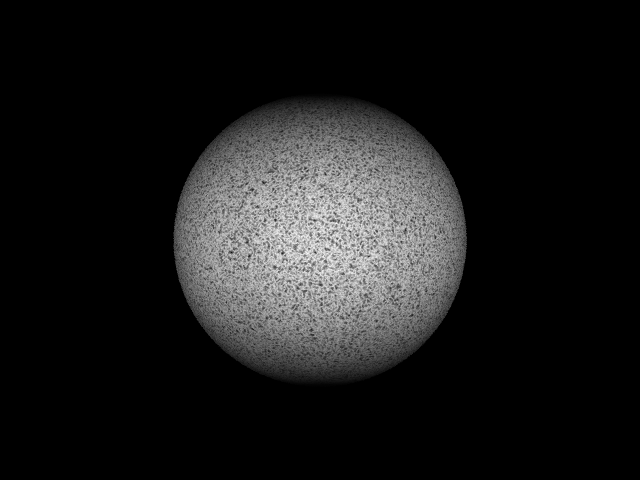
\includegraphics[scale=0.5]{./proceduralStone.png}
 % proceduralOrganic.png: 640x480 pixel, 72dpi, 22.58x16.93 cm, bb=0 0 640 480
 \caption{Piedra tipo Granito Procedural}
 \label{fig:figure4}
\end{figure}

\subsection{Madera}

Para obtener madera, utilizamos la función de ruido sin ningún agregado, pero
al resultado obtenido le realizamos una correción para obtener los anillos que
nos dan la impresión de un árbol.  Esta corrección es la resta de la parte
entera del ruido que se puede observar en la ecuación \ref{resta}.


\begin{equation}
 Noise = Fnoise(p) + \frac{1}{2} Fnoise(2p) + ...
\end{equation}

\begin{equation}
\label{resta}
 Noise = Noise - (int) Noise
\end{equation}

De esta manera, obtuvimos como resultado lo que se puede observar en la figura
\ref{fig:figure5}.

\begin{figure}[h!]
 \centering
 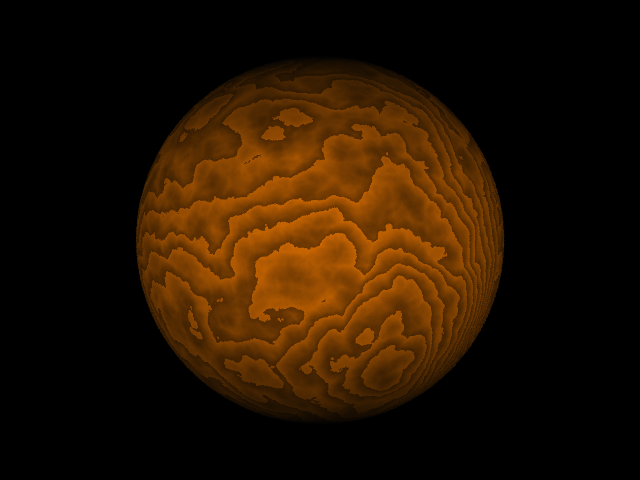
\includegraphics[scale=0.5]{./proceduralWood.png}
 % proceduralOrganic.png: 640x480 pixel, 72dpi, 22.58x16.93 cm, bb=0 0 640 480
 \caption{Madera Procedural}
 \label{fig:figure5}
\end{figure}

\subsection{Mármol}

Para obtener mármol, utilizamos la función propuesta por Ken Perlin.  Este
consiste en:

\begin{equation}
 sin ( x + sum (\frac{1}{f} |noise| )) = sin( x  +  |noise(p)| + \frac{1}{2}
|noise(2p)| + ...)
\end{equation}

Donde el resultado obtenido se observa en la figura \ref{fig:figure6}.

\begin{figure}[h!]
 \centering
 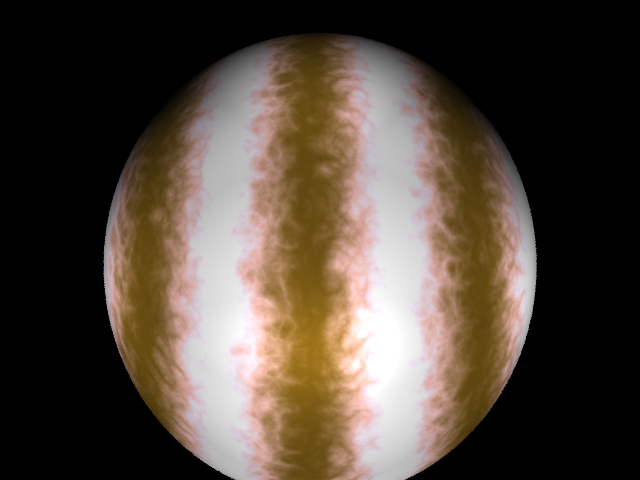
\includegraphics[scale=0.5]{./proceduralMarble.png}
 % proceduralOrganic.png: 640x480 pixel, 72dpi, 22.58x16.93 cm, bb=0 0 640 480
 \caption{Mármol Procedural}
 \label{fig:figure6}
\end{figure}


\section{Representación}
\label{representacion}

Para representar los distintos tipos de shaders nuevos, nos basamos en la
definición de $sunflow$. A continuación mostraremos un ejemplo de una
definición y luego indicaremos las distintas opciones que pueden ser utilizadas.

\begin{verbatim}
shader {
   name fire0
   type fire
   depth 5
   diffuse_initial { "sRGB nonlinear" 1.000 1.000 0.000 }
   diffuse_final { "sRGB nonlinear" 1.000 0.15000 0.000 }
}                         
\end{verbatim}

Este ejemplo, corresponde a la definición de un shader que simula el fuego.
Donde $name$ es el nombre que le daremos al shader, en este caso $fire0$, el
típo de $shader$ está dado por $type$, donde las opciones son $fire$, $water$,
$organic$, $wood$, $marble$ y $stone$.  Luego tenemos la profundidad con la que
queremos que sume, esto es la cantidad de veces que va a sumar ruido, dado por
el parámetro $depth$ que en este caso está con valor 5.  Por último, los
valores de $diffuse_initial$ y $diffuse_final$ determinan el color de comienzo
y de final para el shader.  En este caso, los colores iniciales y finales son
amarillo y rojo como se puede observar en la figura \ref{fig:figure1}

\begin{center}
  \begin{tabular}{ | l || c | r | }
    \hline                       
    Tipo & Color RGB Inicial & Color RGB Final \\
    \hline
    \hline
    fire & (1.0, 1.0, 0.0) & (1.0, 0.150, 0.0) \\
    water & (0.0, 0.0, 0.50) & (0.0, 0.50, 0.50) \\
    marble & (0.466, 0.340, 0.066) & (0.914, 0.706, 0.633) \\
    wood & (0.392, 0.196, 0.0) & (0.784, 0.392, 0.0)
\\
    organic & (0.30, 0.30, 0.0) & (1.0, 1.0, 1.0) \\
    stone & (0.20, 0.20, 0.20) & (1.0, 1.0, 1.0) \\
    \hline  
  \end{tabular}
\end{center}

Los valores presentados en la tabla que precede, son los valores recomendados
para obtener los colores con los que se presentaron los resultados obtenidos
con este desarrollo.


\section{Conclusión}
\label{conclusiones}

\end{document}
